%%%%%%%%%%%%%%%%%%%%%%%%%%%%%%%%%%%%%%%%%%%%%%%%%%%%%%%%%%%%%%%%%%%%%%%%%%
\documentclass[a4paper]{article}
\usepackage{fullpage}
\usepackage{color}
\usepackage[table]{xcolor}
\usepackage{listings}

\definecolor{darkWhite}{rgb}{0.95,0.95,1.00}

\lstset{
aboveskip=3mm,
belowskip=-2mm,
backgroundcolor=\color{darkWhite},
basicstyle=\footnotesize,
breakatwhitespace=false,
breaklines=true,
captionpos=b,
commentstyle=\color{red},
deletekeywords={...},
escapeinside={\%*}{*)},
extendedchars=true,
framexleftmargin=16pt,
framextopmargin=3pt,
framexbottommargin=6pt,
frame=tb,
keepspaces=true,
keywordstyle=\color{blue},
language=C,
literate=
{²}{{\textsuperscript{2}}}1
{⁴}{{\textsuperscript{4}}}1
{⁶}{{\textsuperscript{6}}}1
{⁸}{{\textsuperscript{8}}}1
{€}{{\euro{}}}1
{é}{{\'e}}1
{è}{{\`{e}}}1
{ê}{{\^{e}}}1
{ë}{{\¨{e}}}1
{É}{{\'{E}}}1
{Ê}{{\^{E}}}1
{û}{{\^{u}}}1
{ù}{{\`{u}}}1
{â}{{\^{a}}}1
{à}{{\`{a}}}1
{á}{{\'{a}}}1
{ã}{{\~{a}}}1
{Á}{{\'{A}}}1
{Â}{{\^{A}}}1
{Ã}{{\~{A}}}1
{ç}{{\c{c}}}1
{Ç}{{\c{C}}}1
{õ}{{\~{o}}}1
{ó}{{\'{o}}}1
{ô}{{\^{o}}}1
{Õ}{{\~{O}}}1
{Ó}{{\'{O}}}1
{Ô}{{\^{O}}}1
{î}{{\^{i}}}1
{Î}{{\^{I}}}1
{í}{{\'{i}}}1
{Í}{{\~{Í}}}1,
morekeywords={*,...},
numbers=left,
numbersep=10pt,
numberstyle=\tiny\color{black},
rulecolor=\color{black},
showspaces=false,
showstringspaces=false,
showtabs=false,
stepnumber=1,
stringstyle=\color{gray},
tabsize=4,
title=\lstname,
}


%%%%%%%%%%%%%%%%%%%%%%%%%%%%%%%%%%%%%%%%%%%%%%%%%%%%%%%%%%%%%%%%%%%%%%%%%%
\usepackage{tikz}
\usetikzlibrary{arrows,automata,shapes}
\usepackage[]{graphicx}
\usepackage[]{color}
\usepackage{alltt}
\usepackage[T1]{fontenc}
%%\usepackage{luipsum}
\usepackage{tikz}
%\usetikzlibrary{shapes,arrows}
%\usetikzlibrary{intersections}
\usepackage[utf8]{inputenc}
\usepackage[french]{babel}
\usepackage{graphicx}
\usepackage{amsmath}
%\graphicspath{{./image/}}
\usepackage[left=3cm,right=3cm,top=2cm,bottom=2cm]{geometry}
\usepackage{hyperref}
\usepackage{float} 
\begin{document}



\label{sec:title}
\thispagestyle{empty}

\noindent

\includegraphics[width=0.4\textwidth]{Pictures/ENSEIRB.png}

\vspace{\stretch{1}}


\vspace{\stretch{1}}

\noindent\rule{\textwidth}{1pt}
\begin{flushright}
  \Huge
  \textbf{ Acting Shooting Star }


  \large 
  \textsl{Projet de programmation en langage Racket}

\end{flushright}
\noindent\rule{\textwidth}{1pt}

\vspace{\stretch{1}}

\large
\noindent\textbf{Auteurs  : } \textup{Mohamed Amghar, Salim Bekkari, Mouhcine  El Hammadi, Hamza Mechach}\\ \\
\noindent\textbf{Encadrant :} \textup{Myriam Desainte-Catherine}


\normalsize

\vspace{\stretch{1}}


\vspace{\stretch{1}}


\begin{center}
  Première année, Semestre 6, Filière informatique, ENSEIRB-MATMECA\\
  Date: \today
\end{center}

\vspace{\stretch{1}}



%%%%%%%%%%%%%%%%%%%%%%%%%%%%%%%%%%%%%%%%%%%%%%%%%%%%%%%%%%%%%%%%%%%%%%%%%%%%%
\newpage
\tableofcontents
\pagebreak
%%%%%%%%%%%%%%%%%%%%%%%%%%%%%%%%%%%%%%%%%%%%%%%%%%%%%%%%%%%%%%%%%%%%%%%%%%%%%

\section{Introduction}
Ce projet est notre deuxième projet de programmation pour la première année en école d'ingénieur Enseirb-Matmeca, et il est notre premier projet de programmation avec le langage Racket. Voici une présentation brève qui le décrit :
\subsection{Présentation brève du projet}
%c est un jeu en racket
Acting Shooting Star est un projet qui consiste en l'implémentations d'un \textbf{jeu} avec le langage de programmation \textbf{Racket} en utilisant les différentes techniques de la \textbf{programmation fonctionnelle}. Son but ultime est de se familiariser avec Racket qui est un langage de programmation de la famille \textbf{Lisp}, d'appliquer et de renforcer les connaissances acquises dans le cours de la programmation fonctionnelle.

\subsection{Description du projet}\label{description}
%comme labri
Le jeu que nous essayons de programmer est similaire au jeu connu \textbf{Shoot'em up} ou le jeu \textbf{Terminal phase} présenté brievement dans le site \href{https://dustycloud.org/blog/terminal-phase-prototype/}{\textbf{suivant}}.

Ce projet est basé sur la notion des acteurs. Il s'agit d'un modèle de programmation concurrent construit sur l'idée d'un monde remplit d'acteurs échangeant des messages, et ayant chacun un état propre. En effet, notre jeu contiendra plusieurs acteurs (pour vivifier le jeu) qui peuvent communiquer entre eux, et recevoir des messages de la part d'un serveur. Le serveur est censé garantir le bon déroulement du jeu, et préciser l'état de chaque acteur à chaque instant, il est donc le moteur principale du jeu.

Pour simplifier par rapport au modèle de programmation cité ci-dessus, nous allons considérer que les acteurs se mettent à jour de manière synchronisée. Une horloge globale découpe le temps en intervalles (autrement dit: tick).\\ Au début d'un intervalle de temps, les acteurs n'ont aucun message en attente (état initiale). Ils reçoivent un ensemble de messages pendant cet intervalle sans autre modification. A la fin de l'intervalle de temps, ils vident leur boîte de message et se mettent à jour en fonction de ce qu'ils ont reçu.\\
Pratiquement, la bibliothèque \textbf{lux} présente plusieurs fonctions qui nous serons utile :
\begin{itemize}
    \item[*] \textbf{word-fps}
    \item[*] \textbf{word-label}
    \item[*] \textbf{word-event}
    \item[*] \textbf{word-output}
    \item[*] \textbf{word-tick}
\end{itemize}

La documentation de ces fonction est dans le site \href{https://docs.racket-lang.org/lux/index.html?q=world-tick}{\textbf{suivant}}, dans la partie 2.

\subsection{Problématique}
La problématique qui se pose donc est : \\
Comment peut-on incrémenter la totalité du jeu en utilisant les principes de la programmation fonctionnelle ? \\
Comment peut-on animer le jeu et le programmer de telle façon qu'il soit jouable ?

\subsection{Organisation du projet}
%parler des questions (voir labri)
Le sujet du projet \href{https://www.labri.fr/perso/renault/working/teaching/projets/2019-20-S6-Scheme-Actors.php}{\textbf{ici}} présente différentes questions numérotées de 1 à 8, et qui permettent une bonne approche à la programmation de ce jeu.

Les questions sont dans l'ordre suivant :
\begin{enumerate}
    \item Écrire le code nécessaire pour définir des acteurs et des messages. Les messages sont libres. Les acteurs sont censés posséder au minimum une position dans l'espace. Chaque acteur doit pouvoir répondre au message '(move x y), et se déplacer de (x,y). Ils sont censés implémenter les fonctions suivantes :
    \begin{itemize}
        \item[->] (actor-location actor)
        \item[->] (actor-send actor msg)
        \item[->] (actor-update actor)
    \end{itemize}
    \item Écrire le code nécessaire pour manipuler un ensemble d'acteurs évoluant sur un tick d'horloge. Pour commencer, il est conseillé de construire une structure world rassemblant l'ensemble des acteurs en jeu. À chaque tick d'horloge, cette structure pourra envoyer un message de déplacement à chaque acteur en jeu.
    \item Écrire le code nécessaire pour visualiser la position des acteurs en jeu à chaque instant.
    \item Adapter le code de manière à permettre aux acteurs de créer de nouveaux acteurs. (Pour introduire la notion de "Fire")
    \item Adapter le code de manière à permettre de gérer les collisions entre acteurs
    \item Adapter le code de manière à permettre aux acteurs d'envoyer des messages aux autres acteurs.
    \item Adapter le code de manière à permettre de remonter le temps.
    \item Animer le tout à l'aide de la bibliothèque Lux.
\end{enumerate}
%parler un peu des taches par personnes
\subsection{Outils de communication}
Nous avons trouvé que l'outil le plus facile à utiliser et qui assure la communication entre nous était messanger (Facebook). Celui-là nous a permis d'envoyer des messages sans avoir une bonne connexion, ce qui était louable dans notre cas. \\Nous nous partagions les taches, et nous faisions des séances hebdomadaires pour voir son déroulement du projet et partager des remarques et des idées qui nous pourrions être utile.\\
Pour le rapport, nous nous somme partagé un fichier dans "overleaf.com" qui permettait de rédiger le rapport par plusieurs personnes dans le même instant.\\
Notre encadrant, Mme Myriam, organisait des séances hebdomadaires (chaque vendredi) pour voir notre avancement et nous donner des remarques sur le code ou sur le projet de manière générale. Elle avait mis dans notre disposition une salle virtuelle dans le site des conférence \href{https://bigbluebutton.org/}{bigbluebutton}, ce qui nous a été utile spécialement lorsqu'on voulait faire des partage d'écran entre nous.

\subsection{Description du dépôt et des tests de la forge}
Nous avions un dépôt thor dans lequel nous partagions les différentes versions du code. Ce dépôt permettait aussi la visualisation des différentes statistiques de chaque membre du groupe. Il permettait aussi la visualisation des différentes mises à jour du code et les différentes versions téléversés du code ce qui est très utile souvent lorsque nous voulons récupérer une version antérieur du code.\\
Il existe aussi un outil qui permet de tester le code. En effet, un outil de la forge, exécute un ensemble de tests, ce qui permet de tester le projet indépendamment de son ordinateur.

%%%%%%%%%%%%%%%%%%%%%%%%%%%%%%%%%%%%%%%%

\section{Présentation des structures fondamentales}
Nous présentant les structures \textbf{message}, \textbf{actor} et \textbf{world}, et la fonction \textbf{runtime} dans cette partie.
\subsection{La structure message }
%actor, message(+ location) world
Comme déclaré dans la partie \ref{description}, le jeu est basé sur la notion des acteurs qui doivent avoir un état propre et peuvent conserver les messages qu'ils vont recevoir au cours du tick d'horloge.\\
\\
 Pour simplifier, nous avonc pris la structure \textbf{message} de la forme suivante : 
\vspace{0.3cm}
\begin{lstlisting}
(struct message (sender params))
\end{lstlisting}
Tel que :
\begin{itemize}
    \item[-] \textbf{message-sender :} contient l'identifiant de l'acteur qui a envoyé le message.
    \item[-] \textbf{message-params :} une liste qui contient les paramètres du message.\\ Voici les formes des message-params considérées : \textit{(move x y)}, \textit{(collide)}, \textit{(fire)}.
\end{itemize}

\subsection{La structure actor}\label{actor}
Nous considérons les trois types d'acteurs :\\
\textbf{Acteur principal} (primary-actor), c'est l'acteur qui représente le joueur extérieur. C'est l'acteur que nous pouvons manipuler en utilisant les commandes décrites dans \ref{commandes}. I \\
\textbf{Acteurs balles} (actor-fire), c'est les acteurs "Fire" que l'acteur principal crée pour se défendre contre les acteurs adversaires. \\
\textbf{Acteurs adversaires} ce sont les acteurs qui jouent contre l'acteur principal. 


Nous avons décidé de présenter la structure \textbf{actor} de la forme suivante:
\vspace{0.3cm}
\begin{lstlisting}
(struct actor (id color place lives score mailbox))
\end{lstlisting}

Tel que:
\begin{itemize}
    \item[-] \textbf{actor-id :} représente l'identifiant de l'acteur sous forme d'une chaîne de caractères. \\Pour l'acteur principale c'est "momo" (nom choisit aléatoirement). \\Pour les balles c'est "Fire".\\ Mais plus important pour les acteurs adversaires, c'est l'étiquette avec laquelle ils vont être représenté dans le terminal. Par exemple, un acteur adversaire dont actor-id est \verb!"(o _ o)"!, va être représenté dans le terminal (dans le jeu) sous la forme \verb!"(o _ o)"!. Ceci nous a permet de représenter une infinité de formes d'acteurs adversaires sans ajouter à chaque fois une fonction qui affiche l'acteur selon son étiquette actor-id d'une certaine manière. Nous avons même la possibilité de représenter des acteurs de taille plus grande, en superposant plusieurs acteurs de différentes étiquettes, ce qui est pratique et rend le jeu plus jouable. Un exemple concret est la fonction \verb!(bear x y)! dans le fichier src/main.rkt qui donne plusieurs acteurs qui, en se regroupant, forment un "acteur" sous le forme d'un \textbf{ours}.
    \item[-] \textbf{actor-color :} la couleur dont l'acteur va être représenté dans le terminal.\\ Exemples: \verb!'black! , \verb!'yellow! , \verb!'red! , \verb!'green! , \verb!'blue!.
    \item[-] \textbf{actor-place :} représente la position de l'acteur. Elle doit être sous la forme (Place x y) tel que : (struct Place (x y)) est la structure qui définit la position (x: abscisse et y: ordonnée). 
    \item[-] \textbf{actor-lives :} un entier qui représente le nombre de vies restants pour l'acteur.
    \item[-] \textbf{actor-score :} un entier qui représente le score du joueur.
    \item[-] \textbf{mailbox :} une liste des struct message, et représente l'ensemble des messages que l'acteur a reçu pendant le tick d'horloge.
\end{itemize}




\subsection{structure world et fonction runtime} \label{world}
%expliquer world et main
Pour la structure \textbf{world}, nous avons choisit :
\begin{lstlisting}
(struct world (tick fps player list previous-world next-world stop)
        #:methods lux:gen:word
        [(define (word-fps w)      ;; FPS desired rate
           (world-fps w))
         (define (word-label s ft) ;; Window label of the application
           " Our game - Our world ! ")
         (define (word-event w e)  ;; Event Handler
           (match e
             ["a" #f]  ;; Quit the application
	         ["q" (send-msg-left w)]   ;send move msg to left
             ["d" (send-msg-right w)]  ;send move msg right
             ["z" (send-msg-up w)]  ;send move msg up
             ["s" (send-msg-down w)]  ;send move msg down
             ["x" (send-msg-shoot w)] ;send msg to shoot
             ["p" (prev-world w)] ;previous world
             ["n" (nex-world w)] ;next world
             [_ (send-msg-move w)] ;if no event , send move msg to all actors
         ))
         (define (word-output w)      ;; What to display for the application
           (match-define (world tick fps player list previous-world next-world stop) w)
           (show-end (show-fire (show-adversaries (show-primary (car player)) list) (cdr player)) (car player)) ;place at --> life..
         )
         (define (word-tick w)        ;; Update function after one tick of time
           (match-define (world tick fps player list previous-world next-world stop) w)
           (if (or (zero? (actor-lives (car player))) stop)
               w
               (world (+ 1 tick) fps (actor-update (vivify-bullets player list)) (actor-update (runtime player list)) (cons w previous-world) next-world #f))) 
         ])
\end{lstlisting}
Tel que :
\begin{itemize}
    \item[-] \textbf{world-tick :} est le tick de ce world. Chaque world a un tick propre.
    \item[-] \textbf{world-fps :} le nombre d'images par seconde du world.
    \item[-] \textbf{world-player :} est une liste contenant le joueur principale et les acteur "Fire" (les balles).
    \item[-] \textbf{world-list :} est une liste d'acteurs adversaires.
    \item[-] \textbf{world-previous-world :} une liste qui contient les structures world précédentes \textit{(tel que car = le world ayant un tick : world-tick - 1 )}. Elle garantit la technique zippers \href{https://en.wikipedia.org/wiki/Zipper_(data_structure)?fbclid=IwAR1EkA6fp8uKhW7-CCY9jwM4Hn_r0YFGuEccYER7Vhui6xVvU5Lscca5iwY}{\textbf{ici}} pour accéder à la structure world précédente avec une \textbf{complexité en temps constante}.
    \item[-] \textbf{world-next-world :} une liste qui contient les structures world après la remonté du temps \textit{(tel que car = le world ayant un tick : world-tick + 1 )}. Elle garantit l'accès à la structure wold suivante en temps constant. 
\end{itemize}
%runtime

\vspace{0.3cm}

Pour permettre aux acteurs d'envoyer des messages aux autres acteurs, nous inplémontons la fonction \textbf{runtime} : 
\begin{lstlisting}
(define (runtime primary-actors list-actors)
    (cond
      [(null? primary-actors) (move-left list-actors)]
      [(not (null? (collisions (car primary-actors) list-actors))) (runtime (cdr primary-actors) (append (map (lambda (x) (actor-send x (message (actor-id (car primary-actors)) (list (quote collide))))) (collisions (car primary-actors) list-actors)) (alive (car primary-actors) list-actors)))]
      [else (runtime (cdr primary-actors) list-actors)]))
\end{lstlisting}
En effet, cette fonction prend une liste contenant l'acteur principale et les acteurs "Fire" (primary-actors), et les permet d'envoyer des messages (de type collide) aux acteurs adversaires (list-actors). Elle retourne la liste des nouveaux acteurs adversaires (les acteurs encore en vie). 

%%%%%%%%%%%%%%%%%%%%%%%%%%%%%%%%%%%%%%%%
\section{Affichage et gestion des acteurs}
Nous expliquons dans cette partie les différentes fonctions qui nous ont aidé à implémenter le projet. Ils s'agit des fonctions qui permettent la manipulation d'un acteur, et les fonctions d'affichage.
\subsection{Fonctions manipulant un acteur}
%voir labri + runtime
Parmi les fonctions primordiales qui nous avons permis de manipuler les acteurs, nous citons : \verb!actor-location!, \verb!actor-send!, \verb!move-actor!, \verb!actor-update!, \verb!show-primary!, \verb!create-actors!..\\ Elles sont expliquées dans la page suivante.

\begin{lstlisting}
(define (actor-location act)
  (actor-place act))
\end{lstlisting}
Cette fonction prend un acteur act, et retourne la position de cet acteur.

\begin{lstlisting}
(define (actor-send act msg)
  (struct-copy actor act [mailbox (cons msg (actor-mailbox act))]))
\end{lstlisting}
Cette fonction prend un acteur act et un message msg et retourne un nouvel acteur dont la liste de messages contient le message msg.

\begin{lstlisting}
(define (move-actor act x y)
  (struct-copy actor act [place (Place (+ (Place-x (actor-location act)) x) (+ (Place-y (actor-location act)) y))]))
\end{lstlisting}
Cette fonction, très utile, prend un acteur act dont la position est (old-x, old-y), un abscisse x et un ordonnée y et retourne un nouvel acteur dont la position est (old-x + x, old-y + y).

\begin{lstlisting}
(define (actor-update-elem act)
  (cond
    [(empty? (actor-mailbox act)) (list act)]
    [(fire? (car (actor-mailbox act))) (append (list (rm-car-mailbox act)) (create-actors act))]  
    [(mov? (car (actor-mailbox act))) (actor-update-elem (struct-copy actor act [place (update-actor-location act)] [mailbox (cdr (actor-mailbox act))]))]
    [(collide? (car (actor-mailbox act))) (sub-life act)]
    [else (actor-update-elem (rm-car-mailbox act))]))
    
(define (actor-update list-actors);
  (cond
    [(null? (cdr list-actors)) (actor-update-elem (car list-actors))]
    [else (append (actor-update-elem (car list-actors)) (actor-update (cdr list-actors)))]))
\end{lstlisting}
Tout d'abord, nous avons créer une fonction (actor-update-elem act) qui fait lamise à jour d'un acteur (selon sa boite aux lettres), et retourne une liste contenant cet acteur (retourne une liste pour traiter le cas du message 'fire dont lequel on rajoute un acteur). Cette fonction nous a été utile lors de l'implémentation de actor-update. En effet, il suffit d'applique actor-update-elem sur chaque acteur, et rassembler les listes retournées par cette fonction.
\\La fonction actor-update prend une liste d'acteurs ayant chacun des messages, et retourne une nouvelle liste d'acteurs dont chacun est mis à jour selon sa boite au lettres "mailbox".
\newline En effet, elle permet de gérer les messages suivants:
\begin{itemize}
    \item \textbf{message (fire)} : ajoute donc dans la liste retourné un acteur "Fire" (balle). \texttt{Il est donc possible que les acteurs créent de nouveaux acteurs.}
    \item \textbf{message (move x y)} : retourne un acteur de nouvelle place (old-x + x, old-y + y).
    \item \textbf{message (collide)} : décrémente une vie des vies de l'acteur recevant ce message. \texttt{Nous parlons donc des collisions.}
\end{itemize}

\begin{lstlisting}
(define (create-actors act)
  (list (actor "Fire" (quote none) (Place (+ (Place-x (actor-location act)) 1) (Place-y (actor-location act))) 1 0 '())))
\end{lstlisting}
Cette fonction prend un acteur et retourne une liste construit d'un acteur "Fire" (balle) placé devant l'acteur act.

Tout ces cinq fonctions (\verb!actor-location!, \verb!actor-send!, \verb!move-actor!, \verb!actor-update!, \verb!create-actors!) n'introduisent \textbf{aucun effet de bord}.


\subsection{Fonctions d'affichage}
\begin{lstlisting}
(define (show-primary act)
  (raart:matte-at term-cols term-rows
                  (Place-x (actor-location act))
                  (Place-y (actor-location act))
                  (raart:bg (quote red) (raart:text ">-"))))
\end{lstlisting}
Cette fonction prend un acteur (l'acteur principal) et retourne un raart qui décrit cet acteur (nous avons choisit le texte ">-" en couleur rouge) 


\begin{lstlisting}
(define (show-adversaries intit-rart list)
  (cond
    [(null? list) intit-rart]
    [(< (Place-x (actor-location (car list))) 0) (show-adversaries intit-rart (cdr list))]
    [else (show-adversaries (place-at intit-rart (Place-y (actor-location (car list))) (Place-x (actor-location (car list))) (raart:bg (actor-color (car list)) (raart:text (actor-id (car list)))))
                            (cdr list))]))
\end{lstlisting}
Cette fonction prend un raart et une liste d'acteurs (acteurs adversaires), et retourne un nouvel raart contenant tout les acteurs de la liste (chaque acteur est décrit par son actor-id comme précisé dans \ref{actor}).
Voici une image qui illustre ce que nous venons de dire:
\begin{figure}[H]
    \centering
    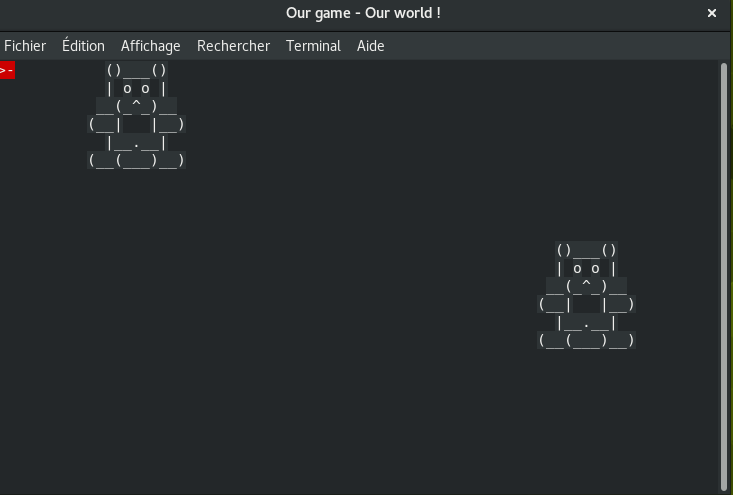
\includegraphics[scale=0.3]{Pictures/bear.png}
    \caption{Figure illustrant les différent types/tailles d'acteurs}
    \label{bear}
\end{figure}


\begin{lstlisting}
(define (show-fire intit-rart list)
  (cond
    [(null? list) intit-rart]
    [else (show-fire (place-at intit-rart (Place-y (actor-location (car list))) (add1 (Place-x (actor-location (car list)))) (raart:text "-->"))
                     (cdr list))]))
\end{lstlisting}
Cette fonction prend un raart et une liste d'acteurs (acteurs "Fire"), et retourne un nouvel raart contenant tout les acteurs de la liste.

\begin{lstlisting}
(define (show-end intit-rart primary-actor)
  (let ([game-over (place-at (matte term-cols term-rows
                                    (frame
                                     (text " GAME OVER ! ")))
                             (+ (modulo (quotient term-rows 2) term-rows) 1) 
                             (- (modulo (quotient term-cols 2) term-cols) 12)       
                             (raart:text " Press 'p' to go back :) "))])
    (cond
      [(zero? (actor-lives primary-actor)) game-over]
      [else intit-rart])))
\end{lstlisting}
Cette fonction prend un raart et l'acteur principal et selon son état (mort ou vivant) décide de montrer "Game over" ou pas. Elle génère le raart suivant :
\begin{figure}[H]
    \centering
    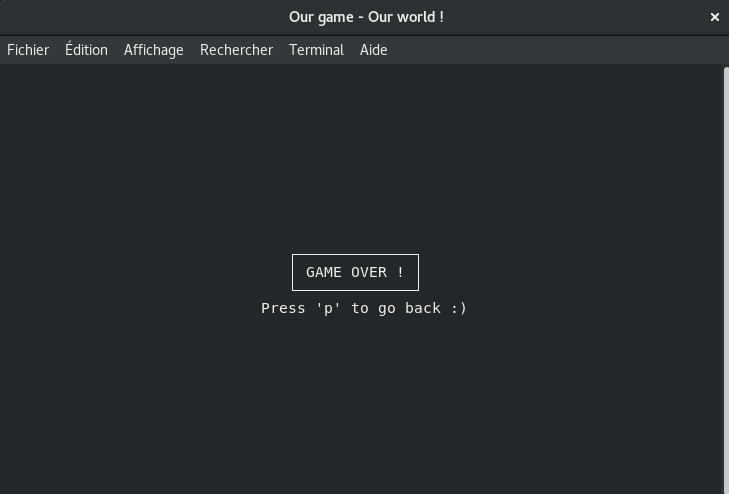
\includegraphics[scale=0.3]{Pictures/game_over.png}
    \caption{La fenêtre qui se génère lorsque le joueur principal n'a plus de vies (0 lives)}
    %\label{fig:my_label}
\end{figure}


\section{Architecture du projet et commandes du jeu}
Le fichier source dans notre dépôt contient cinq fichiers :\\
\textbf{actor.rkt} : contient la structure actor et les différentes fonctions qui permettent la manipulation d'un acteur.\\
\textbf{world.rkt} : contient la structure world et la fonction runtime, ainsi que des fonctions qui permettent la visualisation du jeu.\\
\textbf{main.rkt} : contient la fonction main ainsi que les acteurs qui vont jouer dans la partie.\\
\textbf{tst.rkt} : contient des tests sur les fonctions incrémentés.\\
\textbf{contract.rkt} : contient les contrats.

\subsection{Architecture du projet}
Nous avons choisit la distribution suivante des fichiers pour notre projet :
\begin{figure}[H]
    \centering
    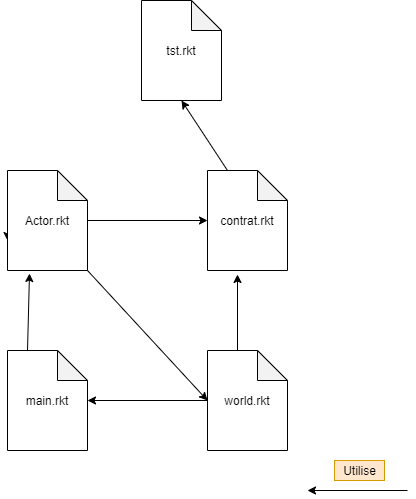
\includegraphics[scale=0.6]{Pictures/architecture.png}
    \caption{L'architecture du projet}
    \label{architecture}
\end{figure}

\subsection{Contrôles/commandes du jeu}\label{commandes}
%expliquer controles du jeu : "a",.."p"..=> remonté du temps
%parler des fonctions send-msg-up ...
Après exécuter la commande "make", le jeu parait (selon la taille du terminal). Nous citons les commandes possibles :
\begin{enumerate}
    \item \textbf{"a"} : permet de quitter le jeu. 
    \item \textbf{"q"} : renvoie une nouvelle structure world où le joueur principal recule par une case (reçoit le message (move -1 0)).
    \item \textbf{"d"} : renvoie une nouvelle structure world où le joueur principal avance par une case (reçoit le message (move 1 0)).
    \item \textbf{"z"} : renvoie une nouvelle structure world où le joueur principal monte par une case (reçoit le message (move 0 -1)).
    \item \textbf{"s"} : renvoie une nouvelle structure world où le joueur principal descend par une case (reçoit le message (move 0 1)).
    \item \textbf{"x"} : renvoie une nouvelle structure world où le joueur principal lance des balles (reçoit le message (fire)).
    \item \textbf{"p"} : renvoie la structure world précédente, et arête le déroulement du jeu jusqu'au clique de n'importe quelle touche.
    \item \textbf{"n"} : renvoie la structure world suivante, et arête le déroulement du jeu jusqu'au clique de n'importe quelle touche.
    \item \textbf{"tout autre touche"} : renvoie la structure world après incrémenter son tick (et faire la mise à jour aux acteurs présents).
\end{enumerate}

%faire des tests et les décrire ici
\section{Discussion}

\subsection{Explication des choix d'inplémentation}
Avant de commencer à coder, nous nous sommes mis d'accord sur les structures. Voici notre raisonnement :
\subsubsection{Structure actor}
Comme déjà mentionné dans \ref{actor}, nous avons choisit d'utiliser \textbf{actor-id} et \textbf{actor-color} pour la représentation de l'acteur. En effet, si l'acteur est mis dans la liste (world-list) des acteurs adversaires, sa représentation dans le terminal sera e tenant compte de ces deux identifiants. Pour \textbf{actor-place} et \textbf{actor-mailbox}, elles sont impératives puisque chaque acteur a une position propre, et doit recevoir des messages. \textbf{Actor-lives} et \textbf{actor-score} améliorent la jouabilité du jeu, et garantissent plus d'idée et de mises à jours sur le jeu (de nouveaux acteurs adversaires à partir d'un certain niveau..).


\subsubsection{Structure world}
Pour la structure world, nous avons choisit de distinguer le joueur principale avec les balles, et les joueurs adversaires, puisque par intuition, on aura dans notre jeu deux parties : la partie des acteurs adversaires qui vont avancer vers le joueur principal, et une l'autre partie constitué de l'acteur principal et les balles.

\subsection{Description des tests}
Pour garantir le bon fonctionnement des fonctions, nous faisons des tests généralement au dessous de chaque fichier. \\
Ceci nous permet d'une part de visualiser (par des flèches) les erreurs en utilisant le programme Drracket. D'autre part, nous avons rencontré un problème avec la forge lorsque nous faisons des tests sur les fonctions qui manipulent la structure world. La forge détecte une erreur. En effet, nous utilisons une fonction dans le fichier world.rkt qui génère les dimensions du terminal pour assurer le bon fonctionnement des fonctions liées à l'affichage. Or dans la forge, il n'existe pas de terminal.  

\subsection{Mis en place des collisions}
La fonction runtime nous permet de gérer les collisions entre acteurs de manière facile. En effet, elle prend la liste des acteurs principaux (acteur principale + balles + balles...), et pour chaque acteur elle parcours la liste des acteurs adversaires et envoie pour chacun d'entre eux qui vérifie une condition (near-collide?) une message de collision. 
\subsection{Mis en place de la remonté du temps}
Pour permettre la remonté du temps en une complexité en temps constante, nous avons ajouter dans la structure world les deux variables previous-world (variable qui conserve les structures-world précédentes) et next-world (qui conserve les structures-world suivantes s'ils existent). Voir partie \ref{world}.
\subsection{Complexités}
%complexité des fonctions de base
Les acteurs que nous manipulons au début de la partie sont l'acteur principale et la liste des acteurs adversaires. L'acteur principale a ensuite la possibilité de créer des acteurs nouveaux (actuers "fire") qui vont lui être utile (se défendre contre les acteurs adversaires), c'est ce qui nous a inspiré de rassembler dans la structure World l'acteur principale et l'ensemble des acteurs "fire" (dans world-player). En prenant donc \textbf{'n'} : le nombre d'acteurs dans un tick d'horloge, et \textbf{'m'} le nombre maximale de messages de chaque acteur dans ce tick.\\

\vspace{0.3cm}
Nous faisons les opérations suivantes (si world-stop est égale à \verb #f ) :
\begin{enumerate}
    \item Incrémenter le world-tick en complexité constante en temps et espace.
    \item Faire envoyer les messages aux acteurs adversaires (de la part des acteurs primaires) par le runtime, et donc récupérer les nouveaux acteurs adversaire. Ceci se fait en complexité en:\\ temps : \textbf{O( n )} car nous parcourons toute la liste des acteurs
    espace : \textbf{O( n )} car nous retournons pour chaque acteur le nouvel acteur mis à jour.
    \item Appliquer la fonction actor-update sur tout les acteurs, qui se fait en complexité en :\\ temps \textbf{O( n x m )}, puisque pour chaque acteur elle parcourt tout ces messages.\\
    espace \textbf{O( n! x m )}, puisqu'on a n acteurs, pour chacun : la fonction actor-update-elem retourne m fois un acteur qui ressemble à celui donné en paramètres (pour chaque message, elle retourne le nouvel acteur mis à jour selon ce message). Et suite à la nature non-terminale de la fonction actor-update, il faudra conserver toujours dans la pile le résultat précédent de la fonction.
\end{enumerate}

La complexité du jeu donc est \textbf{O( n x m )} en temps et \textbf{O( n! x m )} en espace.

\subsection{Améliorations possibles}
Nous parlons des améliorations possibles que nous prévoyons en terme de complexité/temps d'exécusion, et d'attraction du jeu.
\subsubsection{Améliorations sur la complexité du jeu}
Par constatation, nous avons trouvé que le jeu commence à faire des bugs considérables lors de l'ajout des acteurs (en utilisant une centaine d'acteurs). Ceci n'est pas favorable si nous voulons par exemple faire un jeu de plusieurs manches (donc contient plusieurs acteurs). Ce qui nous a poussé de considérer le problème de complexité du jeu. Voici ce que nous avons trouver :\\


%récursivité terminale.
Le temps d'exécution du jeu est encore améliorable. En effet, nous pouvons utiliser des \textbf{fonctions récursives terminaux}. Par exemple dans actor-update, nous pouvons ajouter dans les variables d'entrée de cette fonction une variable qui nous permettra de stocker la liste des acteurs mises à jour. Ainsi, nous n'aurons pas à attendre la pile d'appel pendant l'exécution de cette fonction.\\

%réutiliser les acteurs ---> moins de mémoire;
% # Ceci # Ne dit pas moins de jouabilité
%utiliser actor-score pour mettre à jour les acteurs
Nous avons aussi une idée qui nous permettra de \textbf{diminuer radicalement le nombre d'acteurs} gérés à chaque tick.\\
Tout d'abord, dans notre implémentation actuelle, dans le fichier main.rkt, pour avoir des acteurs adversaires dans différentes positions, nous introduisons de nombreux acteurs adversaires dont plusieurs ont des positions assez éloigné par exemple un abscisse 100 (le terminal ayant par exemple term-cols 15 < 100), et à chaque tick d'horloge ce joueur reçoit un message pour avancer d'un pas vers le joueur principale. A chaque tique d'horloge il faut, donc, manipuler un ensemble de joueurs qui n'apparaissent pas dans le terminal.\\
Or, nous pouvons tout de même prendre un nombre fixe d'acteurs adversaires, par exemple 10 acteurs. Et ne manipuler que ces acteurs pendant tout le jeu. Ceci ne rendra pas le jeu moins jouable. En effet, supposons qu'un acteur parait pour la première fois dans le terminal. Nous le déplacons à chaque tick d'horloge d'un pas comme d'habitude, ceci revient à l'envoyer un message \texttt{(move -1 0)}. Une fois cet acteur arrive à la position dont l'abscisse est 0 (extrémité gauche du terminal), il suffit de lui envoyer un message \texttt{(move term-cols old-y)}, il se retrouvera donc dans l'autre extrémité du terminal et pourra ensuite recevoir les messages \texttt{(move -1 0)} sans sortir du cadre du terminal. Nous pouvons même introduire un aspect aléatoire à sa position de réapparition une fois il arrive à l'extrémité gauche du terminal.\\
Pour plus de diversité, en tenant compte du \textbf{actor-score} du joueur principal, nous pouvons même augmenter le nombres de vies de ces acteurs par exemple. 

\subsubsection{Améliorations sur l'attraction du jeu}
%parler d'ajout des acteurs (more shapes)
Notre implémentation du jeu nous permet d'introduire une variété d'acteurs adversaires. Nous avons introduit une fonction \textbf{(bear x y)} qui génère une liste d'acteurs pour formes un grand "acteur" sous la forme d'un ours. Nous pouvons rajouter plusieurs formes d'acteurs en cherchant des formes/animaux...\\
En effet, nous avons trouver plusieurs formes depuis les caractères ASCII dans ce site \href{https://asciiart.website/}{\textbf{ici}} dont il y a plusieurs formes regroupés par type. 

Nous avons la possibilité de rajouter dans le jeu un acteur qui sera le plus difficile à tuer, et qui aura un nombre de vies assez considérable. Pour sa forme, il pourra prendre une forme d'une scie par exemple.

%parler des améliorations sur affichage (ajouter des fcts qui affichent ..lives..)
Nous pouvons améliorer les fonctions d'affichage. Par exemple dans la remonté du temps, nous pouvons ajouter un petit outil de visualisation qui permet de savoir dans quelle structure world on est.

\subsection{Problèmes rencontrés}
Durant ce projet nous avons rencontré plusieurs problèmes. En fait, il était difficile de gérer deux projets simultanément et d'organiser les taches entre le groupe du travail spécialement dans ces conditions du confinement. Et surtout, nous étions éloignés, et pas tous dans la France. Ce qui a aggravé les problèmes de connections qui existait, et qui ne nous permettais pas de bien communiquer.

\section{Conclusion}
% récapitulatif 
En somme, nous avons construit une version jouable du jeu. Les améliorations sont nombreuses et les idées encore plus. Mais les conditions (COVID-19) n'étaient pas favorables pour permettre la bonne communication entre membres du groupe.\\
Bref, ce projet nous a permis d'améliorer nos connaissances dans le langage Racket et certaines de ces bibliothèque, il nous a aussi permet de se familiariser avec les principes de la programmation fonctionnelle, ses avantages et ses inconvénients. \\
% remerciement
Nous tenons à remercier notre encadrant Madame Myriam Desainte-Catherine, ainsi que notre responsable du projet Monsieur David Renault pour toute aide qu'ils nous ont apporté.
\section{Références}
https://www.labri.fr/perso/renault/working/teaching/projets/2019-20-S6-Scheme-Actors.php \\
https://thor.enseirb-matmeca.fr \\
https://docs.racket-lang.org/
\end{document}
